%%Preambule
\documentclass[12pt,a4paper, french]{article} 
\usepackage[T1]{fontenc}              
\usepackage[utf8]{inputenc}  
\usepackage[french]{babel}
\frenchbsetup{StandardLists=true}
\usepackage{graphicx}
\usepackage{amsmath}
\usepackage[hidelinks]{hyperref}
\usepackage[left=2cm,right=2cm,top=2cm,bottom=2cm]{geometry}
\usepackage[skip=0.17cm]{parskip}
\usepackage{times}
\setlength\parindent{20pt}

%% corps du document
\title{Compte Rendu TP 5 d'instrumentation: Transition du signal, phénomèes de propagation et d'atténuation.}  
\author{Sacha HENAFF/Hadi BOUCHEMA}
\date{}
\begin{document}
    \maketitle
    \tableofcontents
    \section*{Introduction}
    \addcontentsline{toc}{section}{Introduction}
    %%Début intro
    Lors de la transmission d'un signal quel qu'il soit, il faut prêter attention à ses taux d'atténuation
     et de déformation en fonction du signal à transmettre. 
    
     On utilise une ligne, c'est-à-dire un ensemble d'au moins deux conducteurs qui forment un circuit
     fermé entre un générateur (une batterie par exemple) et un récepteur (un électro-aimant par exemple). Bien sûr, 
     ces conducteurs doivent être isolés entre eux.
    
    Au cours de ce TP, nous avons étudié la propagation d'un signal électrique dans une ligne de 
    transmission. Nous allons dans un premier temps caractériser le câble que nous allons utiliser comme la vitesse 
    de transmission du signal dans le câble, ainsi que les coefficients de réflexion et d'atténuation lorsque la ligne 
    de transmission engendre des pertes. 
    
    \subsubsection*{Objectifs du TP:}
    \begin{itemize}
        \item Etudier une ligne sans pertes;
        \item Étudier le phénomène de réflexion et d'atténuation dans différentes configurations.
        \end{itemize}
    %%Fin Intro
    
    
    %%Début première partie
    \begin{center}
    \section{Propagation d'un signal dans une ligne de transmission}
    \end{center}
    
    On étudie la propagation d’un signal dans un câble coaxial décrit comme ceci:
    \begin{figure}[!h]
    \begin{center}
        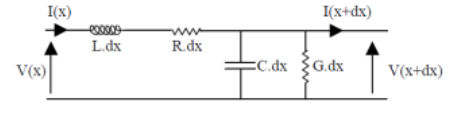
\includegraphics[width=9cm,height=2.5cm]{cablecoax.png}
    \end{center}
    \end{figure}
    
     On a les équations différentielles suivantes qui décrivent l'évolution du courant I(x) et de la tension V(x) le long de la ligne de transmission. 
    \begin{center}
    \begin{equation*}
    \frac{\partial^2V(x,t)}{\partial x^{2}}=LC\frac{\partial^2V(x,t)}{t^2}+(RC+LG)\frac{\partial V(x,t)}{\partial t}+RGV(x,t)
    \end{equation*}
    \begin{equation*}
    \frac{\partial^2I(x,t)}{\partial x^{2}}=LC\frac{\partial^2I(x,t)}{t^2}+(RC+LG)\frac{\partial I(x,t)}{\partial t}+RGI(x,t)
    \end{equation*}
    \end{center}
    
     On représente la ligne de transmission de manière simplifiée comme ceci:
    \begin{figure}[!h]
        \begin{center}
            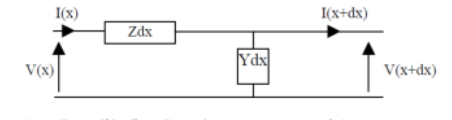
\includegraphics[width=9cm,height=2.5cm]{schemacoax.png}
        \end{center}
    \end{figure}
    On a donc: 
    \begin{center}
    \begin{equation*}
     V(x,t)-V(x+\,dx,t)=ZI(x,t)\,dx
    \end{equation*}
    \end{center}
    
    Donc:
    \begin{center}
        \begin{equation*}
         \frac{V(x,t)-V(x+\,dx,t)}{\,dx}=ZI(x,t)
    \end{equation*}
    \end{center}
    
    Ainsi:
    \begin{center}
    \begin{equation*}
         \frac{\partial V(x,t)}{\partial x}=-ZI(x,t)
    \end{equation*}
    \end{center}
    
    On obtient de même que:
    \begin{center}
    \begin{equation*}
         \frac{\partial I(x,t)}{\partial x}=-YV(x,t)
    \end{equation*}
    \end{center}
    
    Et donc:
    \begin{center}
    \begin{equation*}
            \frac{\partial^2V(x,t)}{\partial x^{2}}=-ZYV(x,t)
    \end{equation*}
    \end{center}
    
    Les solutions de cette équation sont de la forme:
    \begin{center}
    \begin{equation*}
                V(x)=V_{2}e^{\gamma x}+V_{1}e^{-\gamma x}
    \end{equation*}
    \end{center}
    
    On a ici l’onde $V_{2}$ l’onde incidente qui se déplace selon x positif et $V_{1}$ l’onde réfléchie qui se déplace selon les x négatifs. 
    \newpage  
    
    Avec les relations précédentes, on a:
    \begin{center}
        \begin{equation*}
                    V(x)=\frac{1}{Z_{0}}(V_{2}e^{\gamma x}+V_{1}e^{-\gamma x})
    \end{equation*}
    \end{center}
        
    Avec:
    \begin{center}
    \begin{equation*}
        Z_{0}=\sqrt[]{\frac{Z}{Y}}\qquad\text{et}\qquad\gamma = \sqrt[]{(R+\,j L\omega)+(G+\,j C\omega )}
    \end{equation*}
    \end{center}
    
    \subsection{Cas des lignes sans pertes}
    
    On considère ici que la résistance et l'admittance du câble sont nulles, on a donc R=G=0. Ainsi, on a:
    \begin{center}
    \begin{equation*}
        \gamma = j\omega \sqrt{LC}\qquad\text{,}\qquad\alpha =0\qquad\text{et}\qquad\beta =\omega \sqrt{LC}   
    \end{equation*}
    \end{center}
    
    On peut donc calculer la vitesse de propagation du signal qui s’exprime comme:
    \begin{center}
    \begin{equation*}
        \nu_{prop}=\frac{\omega }{\beta }=\frac{1}{\sqrt{LC}}
    \end{equation*}
    \end{center}
    
    \subsection{Discontinuité de l'impédance, phénomène de rélfexion}
    
    On introduit un coefficient de réflexion qui permet de quantifier l’effet d’une discontinuité sur la transmission d’un signal. 
    
    On a donc:
    \begin{center}
    \begin{equation*}
        R=\frac{V_{refl}}{V_{in}}=\frac{V_{1}e^{-\gamma x}}{V_{2}e^{\gamma x}}=\frac{V_1}{V_2}e^{-2\gamma x}\qquad\text{et}\qquad Z(x)=\frac{V(x)}{I(x)}    
    \end{equation*}
    \end{center}
        
    Ainsi:
    \begin{center}
    \begin{equation*}
        Z(x)=Z_0\frac{V_{2}e^{\gamma x}+V_{1}e^{-\gamma x}}{V_{2}e^{\gamma x}-V_{1}e^{-\gamma x}}
    \end{equation*}
    \end{center}
    
    En réécrivant Z(x), on obtient:
    \begin{center}
    \begin{equation*}
        Z(x)=Z_0\frac{1+R}{1-R}\qquad\text{et donc:}\qquad R(x)=\frac{Z(x)-Z_0}{Z(x)+Z_0}
    \end{equation*}
    \end{center}
    
    Dans le cas où, Z est un circuit ouvert (Z(x) est très grand devant Z0), on a $R=1$, si Z(x) est un circuit fermé $(Z(x)=0)$, on a R=-1 et si
     Z est adapté à la ligne $Z(x)=Z_0$, on a $R=0$. 
    
    En effet, si le circuit est ouvert, le coefficient de réflexion vaut 1, toute l’onde est réfléchie car la résistance de l’air tend vers l’infini.
    Sa norme vaut également 1 et la phase est nulle. Si le circuit est fermé, le coefficient de réflexion vaut 1, sa norme vaut donc 1 et la phase vaut $\pi $.
    
    Enfin, si on a une impédance adaptée, c’est-à-dire que Z tend vers Z0, alors le coefficient de réflexion et sa norme sont nuls et la phase ne sera pas définie.
    
    Dans la séance 6 nous nous sommes intéressés au régime de pertes et à la nature des atténuations.
    On peut introduire le coefficient $\alpha_{R}$ qui caractérise les pertes par effet Joule, liées à R et le coefficient $\alpha_{D}$ 
    qui caractérise les pertes diélectriques liées à G. Ces deux
     nouveaux coefficient sont liés par la relation:
     \begin{center}
    \begin{equation*}
            \alpha =\alpha_R+\alpha_D\qquad\text{et}\qquad\alpha \sim \frac{\sqrt{LC}}{2}(\frac{R}{L}+\frac{G}{C})
    \end{equation*}
    \end{center}
    
    Pour déterminer ces pertes on exprime la résistance d’un conducteur homogène ainsi :
    \begin{center}
    \begin{equation*}
                R=\frac{\rho l}{S}
    \end{equation*}
    \end{center}
        
    Ainsi on peut déterminer comment ces pertes résistives évoluent en fonction de la fréquence en exprimant R et $\alpha_R$ en fonction de f. En effet, si à haute fréquence,
     le courant circule à la surface du conducteur sur une épaisseur dite épaisseur de peau, qui s'exprime:
     \begin{center}
    \begin{equation*}
        V=\frac{\sum_{i}\frac{V_i}{R_i}}{\sum_{i}\frac{1}{R_i}}=\frac{V_{saff} R_4}{R_4 + R_5}=\frac{\frac{V_{in}}{R_5}+\frac{V_s}{R_4}}{\frac{1}{R_4}+\frac{1}{R_5}}
    \end{equation*}
    \end{center}
    
    \section{Travaux Pratiques}
    \subsection{Expérience 1}
    
    Dans la première expérience il fallait reproduire le circuit suivant :
    \begin{figure}[!h]
        \begin{center}
            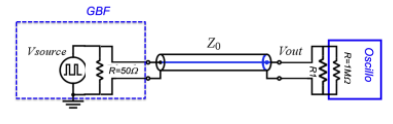
\includegraphics[width=9cm,height=2.5cm]{schemaexp1.png}
        \end{center}
        \end{figure}
    
        Il fallait générer un signal créneau d'amplitude Vpp = 1V et de 
        fréquence 200 kHz. Il a fallu régler l'impédance de sortie du générateur basses
         fréquence à $50\Omega $. On a pris un petit câble coaxial avec des connecteurs BNC de 
         longueur l1 inférieure à 1 mètre. On a alors pu compléter le tableau suivant:
    \begin{center}
        \begin{table}[!h]
        \centering
            \begin{tabular}{|l|l|} \hline
                Configuration & Tension Vpp \\ \hline
                $R_1=1M\Omega$ (circuit ouvert)& 2,10V \\ \hline
                $R_1=50\Omega $ & 1,10V \\ \hline
                $R_1=0\Omega $ (court circuit)&0,40V\\ \hline
            \end{tabular}
        \caption{Résultats de l'expérience 1.}
        \end{table}
        
    \end{center}
    
    Ces résultats s'interprètent de la manière suivante: les 2,10 V de 
    tension correspondent  à la transmission et la réflection du signal dû une imposant
    e résistance (comparable à un circuit ouvert) qui crée une réflection totale de 
    celui-ci qui ne peut passer. En revanche quand $R_1$ vaut $50\Omega $ nous trouvons 
    une valeur presque divisée par deux du cas précédent. Cela est dû au fait qu'ici seul 
    l'onde transmise subsiste majoritairement, la résistance trop faible empêche une
    réflexion importante qui est dans ce cas négligeable. Et enfin dans le cas du court 
    circuit nous nous attendions à trouver une tension nulle. Nous avons émis l'hypothèse
    de la présence d'un résidu, somme de 2 pertes pas tout à fait linéaires.
    
    \subsection{Expérience 2}
    
    On réalise le montage suivant:
    \begin{figure}[!h]
    \begin{center}
            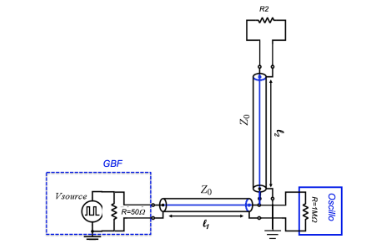
\includegraphics[width=9cm,height=5cm]{schemaexp2.png}
    \end{center}
    \end{figure}
    
    On génère un signal créneau d’amplitude $V_{pp}=1V$ et de fréquence 200kHz, 
    l’impédance de sortie du générateur est fixée à $50\Omega $. La câble $l_1$ mesure moins d’un 
    mètre et le câble $l_2$ mesure plusieurs dizaines de mètres. On mesure la tension aux 
    bornes des câbles coaxiaux et on mesure la tension de ce signal ainsi que l’écart 
    de temps avec lequel il est arrivé. On obtient le tableau suivant. 
    \begin{center}
        \begin{table}[!h]
        \centering
        \begin{tabular}{|c|c|c|c|c|} \hline
            & \multicolumn{2}{c|}{$V_{pp}=1V$, $f=200kHz$, duty $50\%$} &\multicolumn{2}{c|}{$V_{pp}=1V$, $f=2,7MHz$, duty $20\%$}\\ \hline
             Configuration& Tension $V_{pp}$ & Délai $\delta t$& Tension $V_{pp}$ & Délai $\delta t$ \\ \hline
             $R_2=$ouvert & 1,98V & 1000$\mu s$ & 1,78V & 104ns \\ \hline
            $R_2=50\Omega $ &  1,12V & 0s & 1,10V & 240ns\\ \hline
            $R_2=0\Omega $ & 1,98V & 1000$\mu s$& 1,68V&112ns \\ \hline
         \end{tabular}
         \caption{Données de l'expériences 2.}
        \end{table}
    \end{center}
    \medbreak
    
    Dans les configurations 2 et 3, on voit que l'amplitude a doublé, 
    ce qui montre bien que l'on a un coefficient de réflexion de 1 et -1. Dans le 
    circuit 2 il n'y a pas de variation d'impédance, il est donc normal que l'on 
    retrouve une tension proche de celle d'entrée (la petite différence peut être 
    dûe à une résistance interne légèrement différente de $50\Omega $, ce qui modifierait 
    le coefficient de réflexion).
    
    On peut ainsi calculer la longueur du câble coaxial utilisé, on a: 
    \begin{center}
    \begin{equation*}
    v=\frac{2l}{\delta t}=\frac{1}{\sqrt{LC}}\qquad\text{on a donc:}\qquad l=\frac{\delta t}{2\sqrt{(Z_0)^2C^2}}
    \end{equation*}
    \end{center}
    
    On obtient $l=100m$, ce qui est cohérent avec le fait que notre câble
    étati beaucoup plus long que celui de nos camarades.
    
    \newpage
    \subsection{Experience 3}
    
    Pour cette expérience, on utilise un câble le plus long possible pour
     voir de manière plus nette l’atténuation du signal. On réalise le montage suivant:
     \begin{figure}[!h]
        \begin{center}
                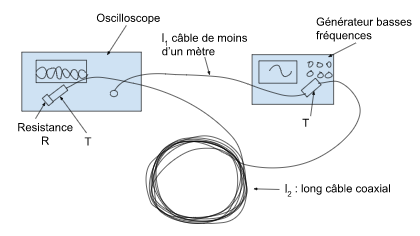
\includegraphics[width=9cm,height=5cm]{schemaexp3.png}
        \end{center}
        \end{figure}
    
    On utilise le montage avec $R=50\Omega $ pour ne pas avoir de discontinuité d’impédance et par conséquent 
    s’affranchir de la réflexion du signal. 
    
    Nous avons ici représenté le cas où nous avons placé la résistance de $50\Omega $.
    Nous avons alors pu faire des mesures des deux signaux $V_{in}$ ($l_1$ câble de moins d’un mètre) et
    $V_{out}$ ($l_2$ câble coaxial de plusieurs dizaines de mètres).
    
    Ensuite nous avons pu tracer le graphe log-log du rapport 
    $-20\log(\frac{V_{out}}{V_{in}})$ en fonction de $\log(f)$.
    \begin{figure}[!h]
        \begin{center}
                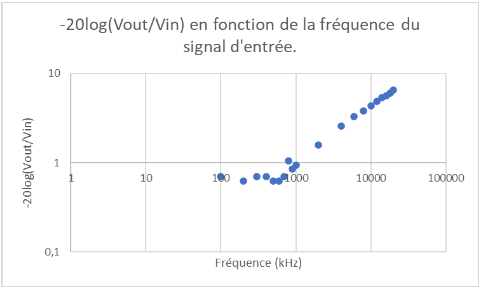
\includegraphics[width=11cm,height=6.5cm]{graphexp3.png}
                \caption{Rapport des signaux d'entrée et de sortie en fonction de la fréquence d'entrée.}
        \end{center}
        \end{figure}
    
    Nous pouvons voir que comme attendu, on voit une partie du graphe où 
    les pertes sont dominées par les pertes diélectriques ($\alpha _d$, dépendance en f) puis une 
    partie du graphe où les pertes sont dominées par les pertes par effet joules ($\alpha_R$ , 
    dépendance en $\sqrt{f}$). Dans ce graphe cette transition survient pour une valeur de 
    fréquence de 1000 Hz. Il s'agit de la fréquence d'utilisation ou fréquence de coupure.
    Lorsque les fréquences deviennent trop hautes, le câble chauffe et les pertes qui 
    dominent deviennent les pertes de dissipation d'énergie par effet joule 
    (dissipation de chaleur).
    
    On peut aussi grâce à ce graphique déterminer la section du câble en déterminant la fréquence du 
    changement de régime de perte (ici environ 600kHz) car on a:
    \begin{center}
    \begin{equation*}
        r=\delta =\sqrt{\frac{2\rho }{\omega \mu }}
    \end{equation*}
    \end{center}
    
    On obtient $r=0,1mm$ ce qui est proche de la valeur mesurée (environ 0,5mm)
    
    \section*{Conclusion}
    \addcontentsline{toc}{section}{Conclusion}
    
    En conclusion dans ce Tp nous avons étudié la manière dont est 
    transmis un signal. Nous avons pu étudier une introduction à l'équation des 
    télégraphistes, la réflexion d'un signal dans un câble coaxial et nous avons 
    pu comprendre les enjeux en termes d'atténuations de celui-ci. Nous avons plus
    précisément pu mettre en place un circuit nous permettant de mesurer ses pertes 
    puis nous avons développé un modèle graphique de ces pertes qui nous a permis de
    diviser ses pertes en deux régimes bien distincts. Nous avons pu les identifier 
    et interpréter ce changement de régime. 
\end{document}
